\documentclass[tikz,border=3pt,convert={density=600,outext=.png}]{standalone}
%\documentclass[tikz,border=3pt]{standalone}

\usepackage[utf8]{inputenc} % utf8 encoding
\usepackage{amsmath} % nice math symbols
     

\usepackage{tikz}
\usetikzlibrary{shapes,positioning,calc,arrows}

\newcommand{\sign}[3]{
	\filldraw[fill=white] ($(0.0,0.2)+(#2,#3)$) -- ($(0.5,1.0)+(#2,#3)$) -- ($(1.0,0.2)+(#2,#3)$) -- cycle;
	\filldraw[fill=black!20] ($(0.0,0.2)+(#2,#3)$) -- ($(0.7,0.0)+(#2,#3)$) -- ($(1.0,0.2)+(#2,#3)$) -- cycle;
	
	\draw[coord_cine] ($(0.5,1.0)+(#2,#3)$) -- ($(0.5,0.13)+(#2,#3)$);
	\draw[coord_cine] ($(0.0,0.2)+(#2,#3)$) -- ($(0.5,0.13)+(#2,#3)$);
	\draw[coord_cine] ($(0.7,0.0)+(#2,#3)$) -- ($(0.5,0.13)+(#2,#3)$);
	\draw[coord_cine] ($(1.0,0.2)+(#2,#3)$) -- ($(0.5,0.13)+(#2,#3)$);
	
	\filldraw[fill=white,fill opacity=0.8] ($(0.0,0.2)+(#2,#3)$) -- ($(0.5,1.0)+(#2,#3)$) -- ($(0.7,0.0)+(#2,#3)$) -- cycle;
	\filldraw[fill=white,fill opacity=0.8] ($(0.7,0.0)+(#2,#3)$) -- ($(0.5,1.0)+(#2,#3)$) -- ($(1.0,0.2)+(#2,#3)$) -- cycle;
	
	\node[sign_comp, fill=red] (s#1_p) at ($(0.0,0.2)+(#2,#3)$) {};
	\node[sign_comp, fill=blue] (s#1_m) at ($(1.0,0.2)+(#2,#3)$) {};
	\node[sign_comp, fill=gray] (s#1_n) at ($(0.5,1.0)+(#2,#3)$) {};
	\node[sign_comp, fill=green!70!black] (s#1_a) at ($(0.7,0.0)+(#2,#3)$) {};
	
	\node[left = of s#1_p] {$p_#1$};
	\node[right = of s#1_m] {$m_#1$};
	\node[right = of s#1_n] {$n_#1$};
	\node[right = of s#1_a] {$a_#1$};
	
	\node[label] at ($(s#1_n)!0.5!(s#1_a)$) {$s_#1$};	
}
% TikZ styles for drawing

\begin{document}
	
	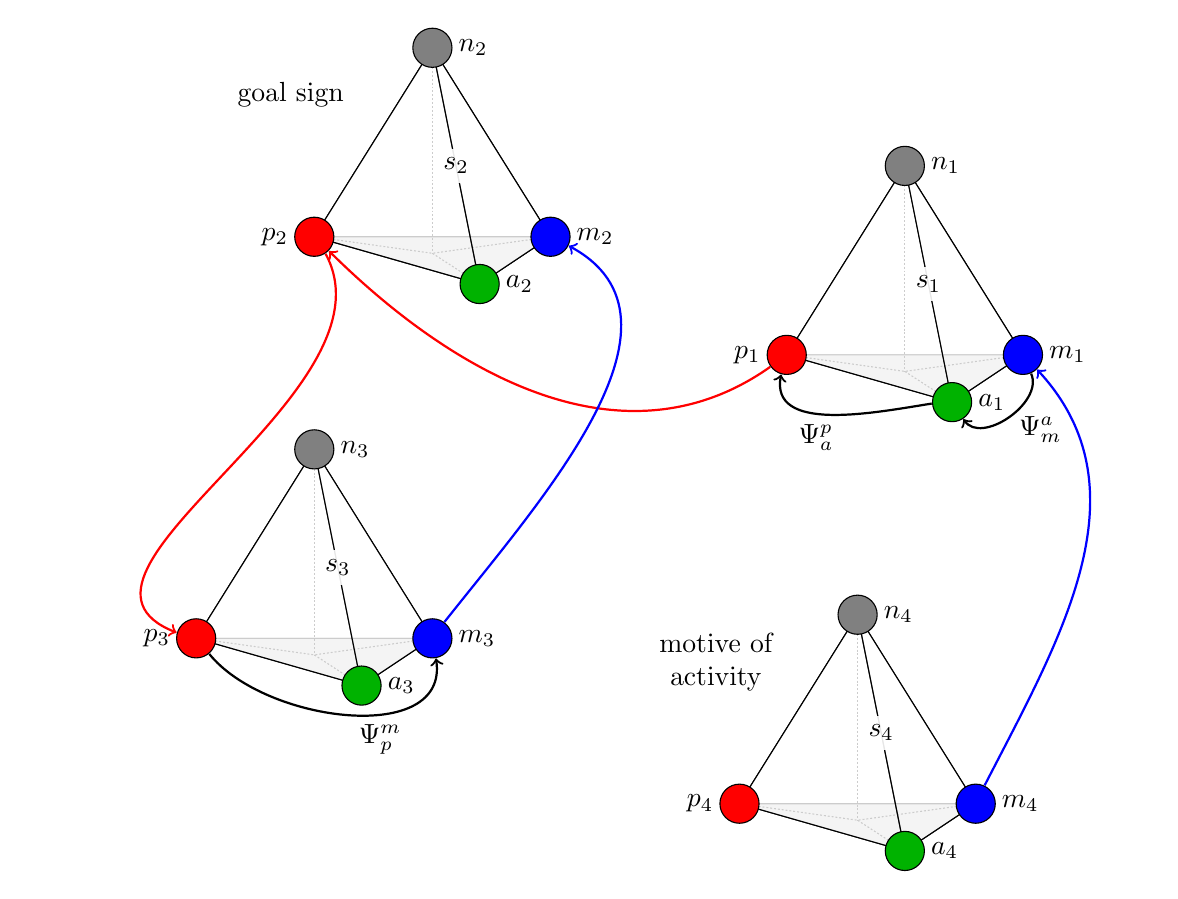
\begin{tikzpicture}[join=round,scale=3.0,node distance = -0.05]
		\tikzstyle{sign_comp}=[draw, circle, scale=1.5];
		\tikzstyle{label}=[align=center,fill=white,opacity=0.9,text opacity=1];
		\tikzstyle{coord_cine}=[dash pattern=on 0.7 off 0.7];
		
		\sign{1}{2.5}{1.2}
		\sign{2}{0.5}{1.7}
		\sign{3}{0.0}{0.0}
		\sign{4}{2.3}{-0.7}
		
		\node[align=center]	at ($(s4_m)+(-1.1,0.6)$) {motive of\\activity};
		\node[align=center]	at ($(s2_m)+(-1.1,0.6)$) {goal sign};
		
		\draw[->,thick, color = red] (s1_p) edge [bend left, out = 50, in = 150] (s2_p);
		\draw[->,thick, color = red] (s2_p) edge [bend left, out = 50, in = -90] (s3_p);
		\draw[->,thick, color = blue] (s3_m) edge [bend left, out = -20, in = -100] (s2_m);
		\draw[->,thick, color = blue] (s4_m) edge [bend left, out = -20, in = -130] (s1_m);
		
		\draw[->,thick] (s1_m) edge [bend left, out = 80, in = 90] node[yshift=4,auto]{$\Psi_m^a$} (s1_a);
		\draw[->,thick] (s1_a) edge [bend left, out = 20, in = 90] node[xshift=-5,auto]{$\Psi_a^p$} (s1_p);
		\draw[->,thick] (s3_p) edge [bend left, out = -50, in = -80] node[yshift=-18,auto]{$\Psi_p^m$} (s3_m);		
	\end{tikzpicture}

\end{document}